
%(BEGIN_QUESTION)
% Copyright 2010, Tony R. Kuphaldt, released under the Creative Commons Attribution License (v 1.0)
% This means you may do almost anything with this work of mine, so long as you give me proper credit

Calculate the appropriate LRV and URV pressures for each of these transmitters to measure two different liquid-liquid interfaces, assuming the span of each transmitter is 10 feet:

$$\includegraphics[width=15.5cm]{i03746x01.eps}$$

Express your answers in units of {\it inches water column} ("W.C. or "H$_{2}$O).

\underbar{file i03746}
%(END_QUESTION)





%(BEGIN_ANSWER)

{\bf Upper transmitter}: \hskip 20pt LRV = $-148.8$ "H$_{2}$O \hskip 50pt URV = $-120$ "H$_{2}$O

\vskip 10pt

{\bf Lower transmitter}: \hskip 20pt LRV = $-120$ "H$_{2}$O \hskip 50pt URV = $-36$ "H$_{2}$O

%(END_ANSWER)





%(BEGIN_NOTES)


%INDEX% Measurement, level: hydrostatic pressure

%(END_NOTES)

